\chapter{REVISIÓN DE LITERATURA}
\label{cap:3}

\section{Definición de términos clave}
\begin{definition}[Precipitación]
 Fenómeno meteorológico que ocurre en sistemas a pequeña escala, caracterizado por la formación de nubes del tipo cúmulus bajo condiciones específicas: presencia de núcleos de condensación, temperaturas cercanas al punto de rocío y un abasto continuo de vapor de agua. A medida que las gotas aumentan de tamaño mediante colisiones, pueden generarse diversas manifestaciones, como lluvia, granizo, nieve, trombas, tornados, rayos y truenos \cite{ahrens2020}.
\end{definition}

\begin{definition}[Lluvia]
    Es la caída de agua procedente de las nubes en estado líquido, sólido y semisólido (\cite{breña2013}).
\end{definition}


El monitoreo es fundamental para la toma de decisiones informadas en la gestión ambiental y otros campos.
\begin{definition}[Monitoreo]
  Es un proceso sistemático y continuo que permite observar, registrar y analizar parámetros específicos para evaluar el estado o cambios en un sistema o fenómeno determinado.(\cite{ciga_monitoreo})
\end{definition}


\begin{definition}[Ciencia Ciudadana]
Es una metodología científica que involucra activamente a la ciudadanía en la generación de conocimiento, permitiendo que personas sin formación científica formal participen en la recolección, análisis e interpretación de datos, contribuyendo así a proyectos de investigación y al fomento de la cultura científica.(\cite{csic_ciencia_ciudadana})
\end{definition}


\begin{definition}[Flutter]
Flutter es un framework de código abierto desarrollado por Google que permite crear aplicaciones nativas de alto rendimiento para múltiples plataformas (iOS, Android, web, escritorio) a partir de una única base de código, utilizando el lenguaje de programación Dart.(\cite{flutter_multiplataforma})
\end{definition}

\begin{definition}[Dart]

Dart es un lenguaje de programación desarrollado por Google, diseñado para crear aplicaciones frontend rápidas y optimizadas, especialmente utilizado en conjunto con Flutter. (\cite{dart})
\end{definition}

\begin{definition}[Widget]

Los widgets son los componentes básicos de la interfaz de usuario de una aplicación de Flutter, y cada widget es una declaración inmutable de una parte de la interfaz. Los widgets se utilizan para describir todos los aspectos de una interfaz de usuario, incluyendo aspectos físicos como texto y botones para diseñar efectos como el relleno y la alineación. (\cite{flutter_multiplataforma})
\end{definition}



\begin{definition}[Firebase]

Firebase es una plataforma de desarrollo de aplicaciones creada por Google que proporciona servicios como bases de datos en tiempo real, autenticación de usuarios, hosting de archivos y funciones de backend sin servidor, facilitando el desarrollo y escalamiento de aplicaciones móviles y web. (\cite{firebase})
\end{definition}


\begin{definition}[Backend]
El backend se refiere a la parte del desarrollo de software que gestiona la lógica de negocio, bases de datos, servidores y APIs, funcionando como la estructura interna que sostiene y conecta los servicios de una aplicación.(\cite{backend})
\end{definition}



\begin{definition}[Frontend]
  El frontend es la capa de una aplicación que interactúa directamente con el usuario, encargándose del diseño, la estructura y la experiencia visual mediante tecnologías como HTML, CSS y JavaScript o frameworks como Flutter para móviles.(\cite{frontend})
\end{definition}


\begin{definition}[GitHub]
  \textit{GitHub} es una plataforma de desarrollo colaborativo que permite a los desarrolladores alojar proyectos, gestionar versiones mediante Git, colaborar en equipos, revisar código y automatizar flujos de trabajo. Su integración con Git permite el control detallado de versiones, ramas y contribuciones en proyectos de software. Además, ofrece funcionalidades como GitHub Actions, Issues, Pull Requests y GitHub Pages, lo que la convierte en un entorno completo para el desarrollo y la gestión de proyectos de código abierto y privado \cite{githubdocs}.
\end{definition}


\begin{definition}[Google Play Console]
  Google Play Console es la plataforma de gestión que permite a los desarrolladores publicar, actualizar, monitorear el rendimiento y administrar la distribución de sus aplicaciones Android en la tienda Google Play.(\cite{googleplayconsole})


\end{definition}

\begin{definition}[Firebase Realtime Database]
Es un servicio de base de datos en la nube que almacena y sincroniza datos entre usuarios en tiempo real, ideal para aplicaciones que requieren actualizaciones inmediatas. (\cite{firebaserealtime})
\end{definition}

\begin{definition}[User Interface (UI)]
  La \textit{interfaz de usuario} (UI, por sus siglas en inglés) es la capa visual e interactiva de una aplicación o sistema digital, diseñada para facilitar la interacción del usuario con las funcionalidades internas del software. Comprende todos los elementos gráficos visibles como botones, formularios, menús, iconos, gráficos y controles que permiten a los usuarios ejecutar tareas específicas. Una UI bien diseñada se enfoca en la usabilidad, accesibilidad, estética y eficiencia, siendo un componente esencial en la experiencia del usuario \cite{shneiderman}.
\end{definition}



\begin{definition}[Material Design]
Material Design es un sistema de diseño desarrollado y respaldado por diseñadores y desarrolladores de Google. Material.io incluye una guía detallada de UX e implementaciones de componentes de UI para Android, Flutter y la web.

La última versión, Material 3, permite experiencias personales, adaptables y expresivas, desde colores dinámicos y accesibilidad mejorada hasta bases para diseños de pantalla grande y tokens de diseño. M3 Expressive va un paso más allá al añadir componentes más flexibles, estilos vibrantes y movimiento totalmente integrado. (\cite{materialdesign2023})
\end{definition}

\begin{definition}[Pluviómetro manual]

El pluviómetro manual es un instrumento utilizado para medir la cantidad de precipitación líquida caída en un lugar específico durante un período determinado. Consiste en un recipiente cilíndrico que recoge el agua de lluvia, la cual se mide posteriormente con una probeta graduada. Este instrumento debe cumplir con las especificaciones establecidas en las normas mexicanas para garantizar la precisión y confiabilidad de los datos obtenidos.(\cite{semarnat_pluviometro})
\end{definition}

Las especificaciones para construir un pluviómetro, ilustradas en la figura \ref{t1}, son las siguientes:
\begin{itemize}
    \item El depósito debe tener una entrada estrecha, suficientemente protegida de la radiación, para reducir al mínimo las pérdidas de agua por evaporación
    \item Este instrumento debe colocarse en lugares abiertos y su área de captación debe permanecer horizontal y a 100 cm del suelo. (\cite{se2013})
\end{itemize}

\begin{figure}[h!]
\centering
  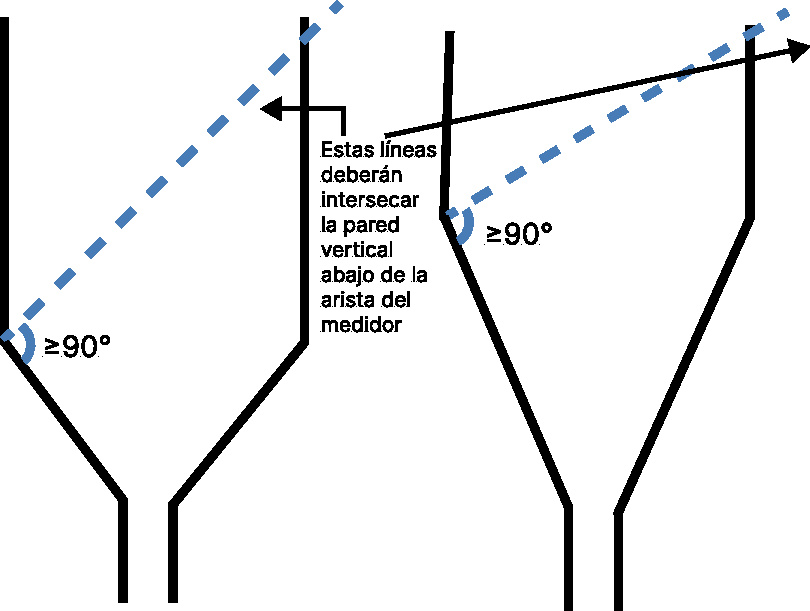
\includegraphics[width=0.5\textwidth]{t1.pdf}
  \caption{Colectaros adecuados para los pluviómetros según la norma NMX-AA-166/1-SCFI-2013 (\cite{se2013})}
  \label{t1}
\end{figure}

% TODO:
% z.tex
% % los antecedentes relevantes al estudio en orden histórico
% \section{Conceptos básicos}
% Las ecuaciones de Naver-Stokes pretenden modelar la evolución de estas cantidades a partir de:
% \begin{itemize}
%     \item La segunda Ley de Newton
%     \item Ley de conservación de la masa y energía
% \end{itemize}
% \subsection{Fuerzas}
% Se consideran fuerzas en fluidos:
% \begin{itemize}
%     \item Variaciones espaciales de presión
%     \item Fuerzas de rozamiento entre moléculas
%     \item Viscosidad
%     \item Fuerza de gravedad
%     \item Fuerzas externas
% \end{itemize}



% \section{Enfoques}
% \subsection{Enfoque Euleriano}
% En el presente estudio se usará éste enfoque,
% \begin{equation}
%     u(x,t) = \left(u_1(x,t),u_2(x,t),u_3(x,t)\right)
% \end{equation}
% La conservación de momento, está dada por:
% \begin{equation}
%     \rho \left(u_t + (u \cdot \nabla)u\right) = -\nabla_{p} + \mu \Delta u + f_e
% \end{equation}
% Esta ecuación se resuelve con la ecuación de continuidad, \textbf{Conservación de masa}
% \begin{equation}
% \rho_t + u\cdot \nabla_{\rho} = 0
% \end{equation}
% \begin{equation}
%     \text{Incompresibilidad}\quad \nabla \cdot u = 0
% \end{equation}


% \subsection{Enfoque Lagrangiano}
% \begin{equation}
%     x = x(a,t)
% \end{equation}
% Es la trayectoria de la partícula que está en la posición del tiempo $t=0$

% Si se analiza el cambio una función $q$ según la trayectora, se calcula con la derivada material:
% \begin{equation}
%     D_tq = q_t + u \cdot \nabla_q
% \end{equation}
% Por la segunda ley de Newton, $D_t(\rho u)=$Fuerza, aunado a la conservación de masa y la incompresibilidad:
% \begin{equation}
%     D_t(\rho) = 0
% \end{equation}

% conservación del momento conservación de la masa
% Se investigó cada parte de la ecuación de Navier-Stokes, su evolución para dos y tres dimensiones, y los últimos trabajos para (tema de tesis) en la Agricultura Vertical


% campo de velocidad de un fluido viscoso incompresible
% flujo de impulso en flujo espacialmente no uniforme



















